%\documentclass[12pt,handout]{beamer}
\documentclass{beamer}
\usepackage{lmodern} % to use fonts in different sizes
\usepackage{xcolor, graphicx, multirow,amsmath,amssymb, bm}
% subcaptions/subfigures
\usepackage[hypcap=true]{subcaption}
% \usetheme{BaylorTheme}
\usepackage[normalem]{ulem}
\usepackage[percent]{overpic}
\usepackage{verbatim}
\newenvironment{metaverbatim}{\verbatim}{\endverbatim}
%% Formatting the Table of Contents
\usepackage{multicol}
\usepackage{booktabs, threeparttable}
\usepackage[backend=biber, style=apa, natbib]{biblatex}
\addbibresource{references.bib}


%\AtBeginSection
%{
%  \begin{frame}{Outline}
%  \begin{multicols}{2}
%  \tableofcontents[currentsection,hideothersubsections]
%  \end{multicols}
%  \end{frame}
%} %% End formatting ToC
%% Coloring
\usetheme[hideothersubsections]{Berkeley}
%\definecolor{baylorgreen}{rgb}{0,.48,.21}
\definecolor{baylorgreen}{cmyk}{.80,0,.63,.75}
%\definecolor{baylorgold}{rgb}{255,188,25}
\definecolor{baylorgold}{cmyk}{0,.21,1,0}
\definecolor{BaylorWhite}{RGB}{255,255,255}
%\definecolor{OliveGreen}{RGB}{0,153,0}
\definecolor{OliveGreen}{cmyk}{.80,0,.63,.75}
\setbeamercolor*{sidebar}{fg=baylorgold, bg=baylorgreen}
% \setbeamercolor*{sidebar}{fg=BaylorWhite,bg=BaylorBlack}
% \setbeamercolor*{sidebar}{fg=BaylorGold,bg=BaylorGreen}
\setbeamercolor*{palette sidebar primary}{fg=black,bg=white}
\setbeamercolor*{palette sidebar secondary}{fg=baylorgold!50!gray, bg=baylorgreen}
% \setbeamercolor*{palette sidebar tertiary}{fg=BaylorGreen!50!black}
% \setbeamercolor*{palette sidebar quaternary}{fg=BaylorGold!10!orange}

\setbeamercolor*{section in sidebar shaded}{parent=palette sidebar secondary}
\setbeamercolor*{subsection in sidebar shaded}{parent=palette sidebar secondary}
\setbeamercolor*{subsubsection in sidebar shaded}{parent=palette sidebar secondary}

% \setbeamercolor*{section in sidebar}{palette sidebar primary}

\setbeamercolor*{section in sidebar}
  	{parent=parent=palette sidebar primary,use={sidebar,section in sidebar shaded},%
   	fg=baylorgreen,bg=baylorgold!80!BaylorWhite}

\setbeamercolor*{subsection in sidebar}
	{parent=palette sidebar secondary,use=section in sidebar,%
   	bg=section in sidebar.bg, fg=section in sidebar.fg} 

\setbeamercolor*{subsubsection in sidebar}
	{parent=palette sidebar secondary,use=section in sidebar,%
   	bg=section in sidebar.bg, fg=section in sidebar.fg}
   	

\setbeamercolor*{palette primary}{use=structure,fg=baylorgold,bg=baylorgreen}

 \usecolortheme[named=baylorgreen]{structure}
 %\usecolortheme{newbears}

\setbeamertemplate{footline}[frame number]

\title[Assessing Local Fit]{Assessing local fit in confirmatory factor models by approximating probabilities}
\author[Padgett]{\Large{R. Noah Padgett}} %
\institute[Not sure]{\large{Baylor University\\
Department of Educational Psychology}\\
}
\date{January 19, 2021}
%% ============================================= %% 
\begin{document}
%% ~~
\frame{\titlepage
\begin{overpic}[scale=.05]{fig/baylorlogo}
     	%\put(12.5,38){
\includegraphics[scale = .05]{baylorlogo}}
%     		%\put(140,-70){\includegraphics[scale=1.5]{masters.jpg}}
%     			%\put(75,30){\includegraphics[scale=.27]{andrich.jpg}}
\end{overpic}
}
%% ~~
\frame{
	\frametitle{A Road-map}
	\tableofcontents[hidesubsections]
}
%% ~~
\section{Introduction to Fit Assessment}
\frame{
	\frametitle{Test Construction and Validity}
	\begin{itemize}
	\item Confirmatory Factor Analysis is commonly used in test construction.
	\item Aim is to provide some construct validity evidence through the measurement model proposed \citep{Bandalos2016}.
		\begin{itemize}
		\item[-] Is there evidence that items commonly measure a construct(s)?
		\item[-] How do items groups into subscales or is there evidence of multidimensionality in some items?
		\item[-] These are a couple of potential questions we aim to address in the test evaluation process.
		\end{itemize}
	\end{itemize}
} % End frame
%%~~
\frame{
	\frametitle{Confirmatory Factor Analysis}
	\centering
	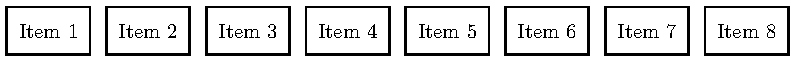
\includegraphics[width= 1\textwidth]{fig/sera_pres_cfa0}
} % end frame
%%~~
\frame{
	\frametitle{Confirmatory Factor Analysis}
	\centering
	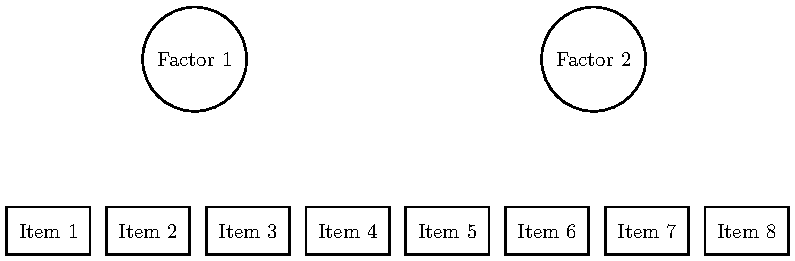
\includegraphics[width= 1\textwidth]{fig/sera_pres_cfa1}
} % end frame
%%~~
\frame{
	\frametitle{Confirmatory Factor Analysis}
	\centering
	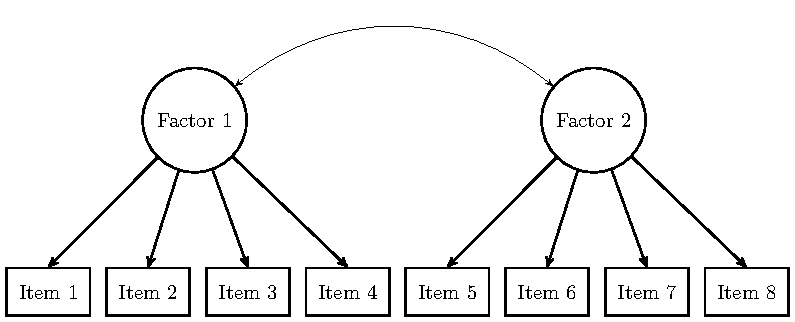
\includegraphics[width= 1\textwidth]{fig/sera_pres_cfa2}
} % end frame
%%~~
\frame{
	\frametitle{Confirmatory Factor Analysis}
	\centering
	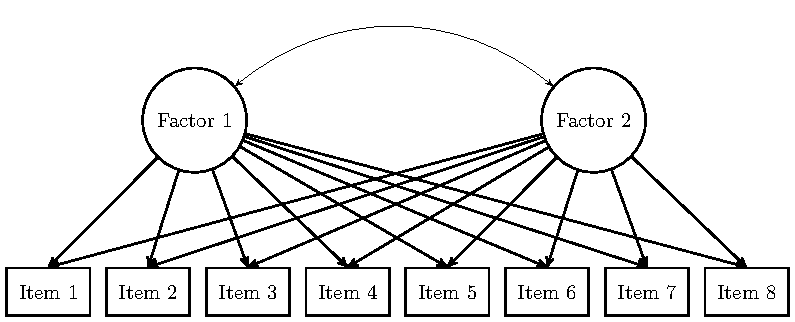
\includegraphics[width= 1\textwidth]{fig/sera_pres_cfa3}
} % end frame
%%~~
\frame{
	\frametitle{Confirmatory Factor Analysis}
	\centering
	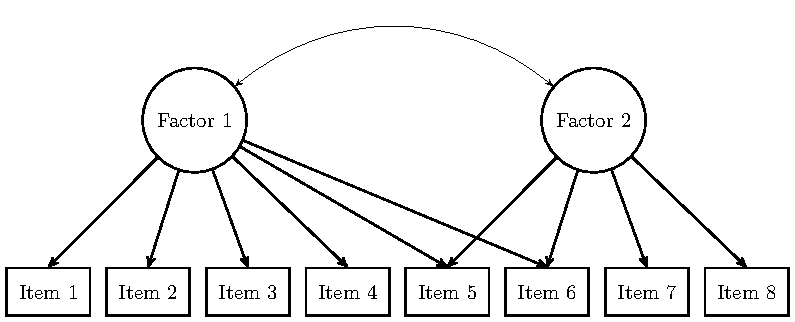
\includegraphics[width= 1\textwidth]{fig/sera_pres_cfa4}
} % end frame
\frame{
	\frametitle{CFA Model Modifcation}
How do you justifiably modify your measurement model?

(pause - this isn't rhetorical)	
} % frame end
%~~
\subsection{Model Fit Assessment}
\frame{
	\frametitle{Global Assessment}
	A \textit{global assessment} of model fit is traditional day by investigating the overall relationship between
	\begin{align*}
	Observed\ &-\ Expected\\
	\mathbf{S} &- {\bm\Sigma}(\hat{\theta})
	\end{align*}
} % end frame
% ~~
\frame{
	\frametitle{Global Assessment Cont.}
	Global assessment is traditionally accomplished using
	\begin{itemize}
	\item $\chi^2$-test of model fit \citep{Bollen1989} (need p. \#)
	\item Comparative Fit Index \citep[CFI; ][]{Bentler1990}
	\item Room Mean Square Error of Approximation \citep[RMSEA; ][]{Browne1992}
	\item Standardized root mean square residual \citep[SRMR; ][]{Bentler1995, Joreskog1981, Maydeu2018}
	\item among others as well.
	\end{itemize}
	A potential pitfall is that these approaches only provide a general overall assessment of model fit and does not inform us where or which relationships are not captured by our model \citep{Steiger2007}.
} % end frame
% ~~
\frame{
	\frametitle{Local Assessment}
	A \textit{local assessment} of model fit refers to assessing model subcomponents or individuals relationship for lack of fit or contribution to inference
	\begin{align*}
	s_{ij} - \sigma_{ij}(\hat\theta)
	\end{align*}
	for observed covariance between items $i$ and $j$ or the contribution of a parameter $\theta$ to the model
}  % end frame
% ~~
\frame{
	\frametitle{Local Assessment Cont.}
	Often, local fit assessment results in suggested modifications to the proposed model. Potential modifications include
	\begin{itemize}
	\item Removing paths or potentially unnecessary relationships
	\item Adding paths or covariances to account for relationships
	\end{itemize}
	
} % end frame
% ~~
\frame{
	\frametitle{Some Approaches to Model Modification}
	\begin{itemize}
	\item Modification Indices \citep{Sorbom1989, Kaplan1989}
	\item Wald Tests \citep{Wald1943, Buse1982}
	\item Likelihood Ratio Tests \citep{Buse1982, Neyman1928}
	\item Model Implied Instrumental Variables \citep{Bollen1995, Bollen2019}
	\end{itemize}
	\begin{center}
	And now...
	\end{center}
} % end frame
% ~~
\frame{
	\frametitle{Some Approaches to Model Modification}
	\begin{center}
	Region of Practical Equivalence Probability Approximation\\
	or\\
	ROPE Probability Approximation
	\end{center}
} % end frame
% ~~
\section{Proposed Probabilistic Approach}
\frame{
	\frametitle{ROPE Probability Approximation}
	\begin{itemize}
	\item The goal is to provide an interpretable metric to evaluate the parameter space of a selected model.
	\item The logic is to evaluate the probability that a parameter is outside a region of the parameter space we (as researchers) determine to provide little inferential benefit.
	\item Taken from exploratory factor analysis, we could define all factor loadings (standardized) that are below 0.32 to too low and our new approach approximates the probability that the loading is greater than 0.32.
	\end{itemize}
} % end frame
% ~~
\frame{
	\frametitle{ROPE Probability Approximation Cont.}
	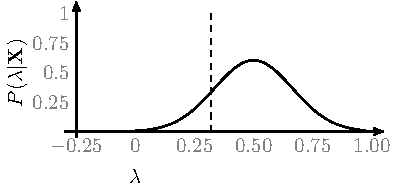
\includegraphics[width=1\textwidth]{fig/probability_curve}
} % end frame
% ~~
\frame{
	\frametitle{Probability Definition}
	\begin{itemize}
	\item The ROPE Probability can be expressed as $\Pr\left(\vert \theta\vert \geq \theta^{\ast} \mid \mathbf{X}\right)$.
	\item For factor loadings, the probability statement is reduced to $\Pr\left(\vert \lambda\vert \geq 0.32 \mid \mathbf{X}\right)$.
	\item For error covariances, the cutoff could be defined by a correlation of 0.25.
	\end{itemize}
} % end frame
% ~~
\frame{	
	\frametitle{Estimation}
	\begin{itemize}
	\item The probability is condition on the data ($\mathbf{X}$).
	\item Traditional frequentist approaches to inference conditions on the parameter, so a Bayesian approach is taken.
	\item To side-step computational complexities, we utilized Laplace's method to approximate the posterior for each parameter.
	\item Briefly, Laplace's method is a Taylor series expansion to approximate any function by a sum of derivatives.
	\begin{align*}
	f(x) &= \sum_{k=0}^{\infty}(\theta - \hat\theta)^kf^{(k)}(\hat\theta)\\
	&\approx \sum_{k=0}^{2}(\theta - \hat\theta)^kf^{(k)}(\hat\theta) + O_2
	\end{align*}
	\end{itemize}
}

\subsection{Guiding Questions}
\frame{
    \frametitle{Research Questions}
\begin{enumerate}
\item Does this new approach provide a noticeably higher probability for parameters from the data generating model compared to true-zero paths?
\item How does the empirical sampling distribution used in the approximation compare to the sampling distribution of the parameters from the true model?
\end{enumerate} 
}%% End Frame
%% =================================== %%
\section{Application to Simulated Data}
%% ~~
\subsection{Fake Data Example}
\frame{
    \frametitle{The Population Model}
    \begin{center}
    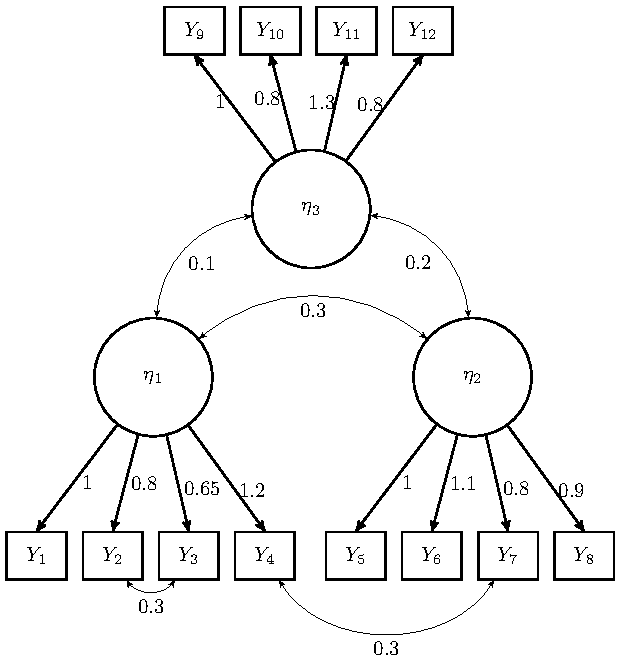
\includegraphics[width = 0.5\textwidth]{fig/sim_factor_structure_values}
    \end{center}
A random sample of 300 was drawn from this population which was adapted from \citep{Bollen2019, Bollen1989}.
} % end frame
% ~~
\subsection{Model Fit without Error Covariances}
\frame{
	\frametitle{Hypothesized Model Fit}
	\begin{itemize}
	\item Model was fit using \texttt{lavaan} \citep{Rosseel2012}.
	\item Model fit summary $\chi^2(51) = 72.8, p = 0.024$
	\item Model does not ``fit'' these data according to a coarse view.
	\item Now, using the ROPE Probability Approximation, we aim to identify where in the model potential modification should be considered.
	\end{itemize}
} % end frame
% ~~
\subsection{ROPE Probability Approximation}
\frame{
	\frametitle{Model Modification Results}
\begin{table}[ht]
\centering
\begin{tabular}{lr}
  \toprule
Parameter ($\theta$) & $\mathrm{Pr}( \mid \theta \mid \geq cutoff)$\\ 
  \midrule
  $\mathrm{cov}(y_7, y_4)$    & 0.810 \\ 
  $\mathrm{cov}(y_3, y_2)$    & 0.461 \\ 
  $\mathrm{cov}(y_9, y_4)$    & 0.233 \\ 
  $\mathrm{cov}(y_4, y_1)$    & 0.160 \\  
  $\vdots$				      & \\
  $\lambda_{19}$              & 0.005 \\
   \bottomrule
\end{tabular}
\end{table}
} % end frame
% ~~
\frame{
	\frametitle{Sampling Distribution of Error Covariances}
	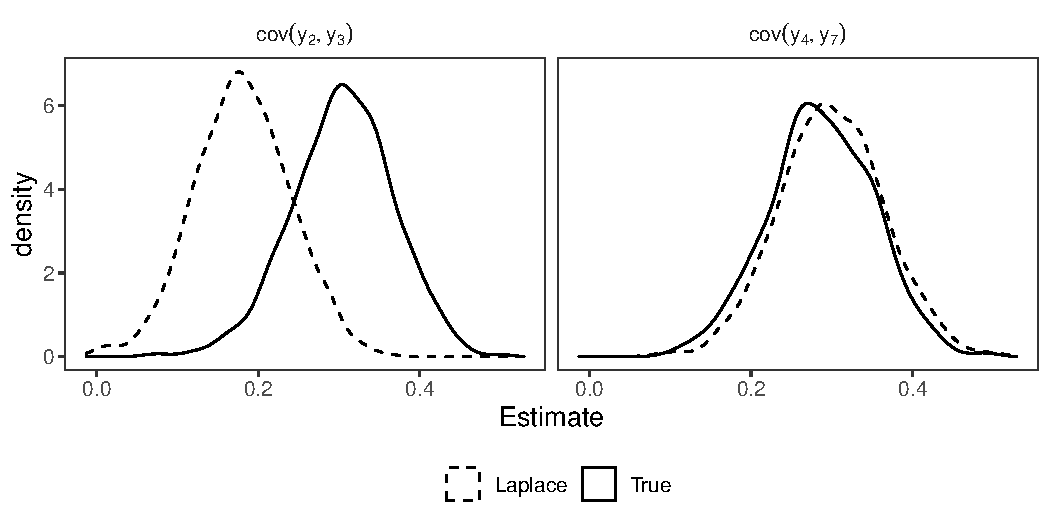
\includegraphics[width=0.9\textwidth]{fig/sampling_dist}
}
\section{Conclusions}
\frame{
	\frametitle{Conclusions}
	\begin{itemize}
	\item The proposed local fit method is an efficient approach to transforming local fit assessment into a probabilistic framework.
	\item The probability is an intuitive approach to assessing whether paths should be modified.
	\item More work needs to be done to evaluate how this approach works in non-simulated datasets.
	\end{itemize}
}
	
\subsection{References}
\begin{frame}[allowframebreaks]
	\frametitle{References}
	\scriptsize
	\printbibliography	
\end{frame}

\end{document}